\documentclass[10pt, a4paper, onecolumn]{scrartcl}
\usepackage{cite}  
\usepackage{times}
\usepackage{amsmath}
\usepackage{amsfonts}
\usepackage{amssymb}
\usepackage{graphicx}
\usepackage{listings}
\usepackage{enumitem} % used for list - no spaces between items
\usepackage[english]{babel} % English language/hyphenation
\usepackage[top=2cm, bottom= 3.2cm, left=2cm, right=2cm, columnsep=0.6cm]{geometry}
\usepackage{color} %red, green, blue, yellow, cyan, magenta, black, white
\definecolor{mygreen}{RGB}{28,172,0} % color values Red, Green, Blue
\definecolor{mylilas}{RGB}{170,55,241}
\usepackage{fancyhdr}
\pagestyle{fancyplain}
\fancyhead{}
\renewcommand{\headrulewidth}{0pt} % Remove header underlines
\fancyfoot[L]{} % Empty left footer
\fancyfoot[C]{} % Empty center footer
\fancyfoot[R]{\thepage} 
\usepackage{tikz}
\usetikzlibrary{shapes.geometric,arrows}

\usepackage{sectsty} % Allows customizing section commands
\sectionfont{\centering\large\textbf}
\subsectionfont{\flushleft\normalsize\normalfont\textbf}
\subsubsectionfont{\flushleft\normalsize\normalfont\textit}
%\allsectionsfont{\centering} % Make all sections centered

\setlength\parindent{0pt} % remove all indentations in document

%----------------------------------------------------------------------------------------
%	BEGIN DOCUMENT
%----------------------------------------------------------------------------------------
\newcommand{\horrule}[1]{\rule{\linewidth}{#1}}

\begin{document}
	
	\title{\normalfont \normalsize
		\textsc{University of Witwatersrand, Department of Electrical Engineering} \\ [10pt]
		\horrule{0.5pt} \\ [10pt]
		\huge Software Requirement Specification for Shopping Route Recommender \\
		\horrule{2pt} \\ [10pt]}
	\author{\textbf{\normalsize{Luka Cakic (671913), Ronen Freeman (386910), Devin Taylor (603956) and Matthew Marsden (609293)}} \\ [10pt]}
	\date {\normalsize \today}
	
	\maketitle
	
	
	\section{Introduction}
	
		\subsection{Purpose}
		
			This document details the Software Requirements Specification (SRS) for the Shopping Route Recommender (SRRec) web application. The document also follows the IEEE standard for SRS documents.\\
			
			Shopping can often prove to be tedious and frustrating when you find out that the shop you are at does not stock or is out of stock of certain products that are on your shopping list. One then needs to go to other shops in the hopes that those shops will have the items not yet ticked off ones shopping list. Even then, the next shop may not have the items and you have to keep going from shop to shop until you finally get all the items needed. There is clearly a need for a more efficient way of finding all the items on your shopping list in the shortest travel time, shortest route or most cost effective route.\\
			
			The purpose of this project is to provide a web application that allows a user to enter their shopping items into a shopping list and in turn provides the user with the ideal route to the nearest stores that will fulfil their needs.
		
		\subsection{Document Conventions}
		
			This document is intended to accompany the SRRec software and should be updated with each update to the web application. This will ensure that the document remains relevant and useful.
		
		\subsection{Intended Audience and Reading Suggestions}
		
			This SRS document is intended for:
			\begin{itemize}
				\item Programmers that want to understand the outlines of how the SRRec web application works and the way in which the software has been implemented.
				\item Project testers to use in order to better their testing strategies since some bugs are easier to find by using an SRS document.
				\item End users of this web application who would like to read about how the SRRec can help them or what it is capable of doing.
			\end{itemize}
		
		\subsection{Project Scope}
		
			SRRec is a web application that is capable of providing a route to all the nearest shops so as to fulfil a users entire shopping list while either following the shortest route, the route with the shortest travel time or the route that will result in minimal total shopping expenses. The shopper can continuously add items to their list and these items are logged to their respective list. When the shopper finally runs the SRRec he/she will obtain their user-determined recommended route of shops to visit in a particular order according to items on their list. The application provides a Graphical User Interface (GUI) with embedded Google Mapsto illustrate this generated route. \\
		
			We assume the following:
			\begin{itemize}
				\item There is already a map of all shopping malls and shops that sell various items that a shopper could add to their list.
				\item Each shop has a database of the items that they stock and their respective prices.
				\item The price of each item is a simple Rand value or indicated by Rand/kilogram, etc.
				\item The SRRec runs on a website with access to the databases of all the shops.
				\item Google maps is available on the website and shows the route from one shopping mall or shop to the next.
			\end{itemize}
			
			The shopper is able to select one of three types of recommendation:
			\begin{itemize}
				\item shortest route.
				\item shortest route for minimal total shopping expenses.
				\item route with shortest travel time.
			\end{itemize}
			
			The shopper will also be able to change their selected recommendation after visiting some shops and eliminating some items from their list. The SRRec can also incorporate stop-overs for coffe, drinks, lunch, etc. At a later stage, the shopper may even be able to provide a price range that they are willing to pay for each item.
		
	\section{Overall Description}
	
		\subsection{Product Perspective}
		
			The Shopping Route Recommender is an application used by consumers to maximise their shopping experience in terms of three preferred optimisations: minimum cost, travel distance and travel time. The consumer is able to log onto a Website or Smartphone application and create a shopping list with a desired route being generated.  Enabling a user to optimise their shopping experience is a potential success from the start, as their daily routines can become more efficiently and effectively undertaken. The application's use is not only restricted to the general public, but can also be used by businesses and companies involved in the stock collection courier service industries. The application is aimed at being user friendly, simple, and interactive with maximum customisation being a priority aspect in order to maximise an individuals needs. 
		
		\subsection{Product Features}
		
			The list of product features below aim to provide an easy-to-use, customizable application interface for all users. 
		
			\begin{itemize}
				\item Interactive shopping list menu.
				\begin{itemize}
					\item add or remove item
				\end{itemize}
				\item Interactive optimisation selection options.
				\begin{itemize}
					\item minimise cost
					\item minimise travel time
					\item minimise travle distance
				\end{itemize}
				\item Interactive shopping area selection options.
				\begin{itemize}
					\item select from a number of suburbs or regions
				\end{itemize}
				\item Interactive route map displaying alternate routes for selection.
				\begin{itemize}
					\item rotate map
					\item slide map
					\item zoom in/out
					\item satellite view
				\end{itemize}
			\end{itemize}
		
		\subsection{User Classes and Characteristics}
		
			The application is aimed for the general public's use as well as certain business industries. 
			
			\begin{itemize}
				\item General Public
				\begin{itemize}
					\item General population wanting to buy their routine shopping list
					\item General population looking for more specific products and their preferred optimised route
					\item Foreign individuals looking for their ideal shopping locations or travel routes
				\end{itemize}
				\item Business Industries
				\begin{itemize}
					\item Courier companies collecting stock or products from various distributors/stores
				\end{itemize}
			\end{itemize}
		
		\subsection{Operating Environment}
		
			Shopping Route Recommender is an application designed to run on the most Web Browsers as well on Google Android and Mac OS X Smartphones. 
			
			\begin{itemize}
				\item Software Requirements
				\begin{itemize}
					\item Internet connectivity
					\item Entry level Smartphone
					\item Mozilla Firefox, Microsoft Edge, Google Chrome, Microsoft Explorer, Safari
				\end{itemize}
				\item Hardware Requirements
				\begin{itemize}
					\item Entry level Smartphone with interactive touch screen
				\end{itemize}
			\end{itemize}
		
		\subsection{Design and Implementation Constraints} 
		
			Shopping Route Recommender is platform independent and is written using PostgreSQL, PHP, Javascript, HTML and CSS. In addition, Google Maps API is implemented for generating the desired optimised shopping route. The accuracy of the generated route and optimisation algorithms is therefore dependent on the accuracy of the Google Maps API utilised. 
		
		\subsection{User Documentation}
		
		   	An application menu will be provided within the application. The menu will house information about the application, the application settings, history tab that is used to store user recent shopping route and a help function that will function as the "user manual" of the application. 
		
		\subsection{Assumptions and Dependencies}
		
			The application is functionally depenedndant on Google Maps API. This API is integral to displaying the shopping route and directions to the user. One assumption is therefore that Google Maps is available on the website and shows the route from one shopping mall or shop to the next. Another functional dependency is that the application depends on the product database of each shop stored in the application's database. It is therefore assumed that each shop has a database of items that they stock as well as their respective prices. These product databases are continuously updated by each of the stores. The application must therefore contain the latest product database updates from each of the stores. The SRR database must therefore be automatically updated once a store has registered an update in its product database. This is an important functional dependency if the application is to be as accurate as possible in terms of product pricing. 
	
	\section{System Features}
	
		Shopping Route Recommender was designed with user experience as its primary concern. As a result of this the product features are simplistic in nature in order to provide the customer with only the essentials.	This section provides a detailed description of each system feature in order to make future system extensions as simple as possible. 
	
		\subsection{System Feature 1 - Adding items to shopping cart}
		\label{featureadd}
		
			\subsubsection{Description}
			
				The Shopping Route Recommender's primary feature is the user's ability to add shopping items to their cart. The user will be able to log into the application and add items to the shopping cart on an add-hock basis. These items will remain in the basket until such time that the user wants to go shopping. 
			
			\subsubsection{Stimulus/Response Sequences}
			
				The user will click in the "Add Items" field at which point a list will be displayed that will contain all previously added items listed one after the other (in the order in which they were added). Within this list the user will be able to complete one of the following actions:
				
				\begin{itemize}
					\item Add a new item - The user will be able to click the "Add new item" button in order to enter a new item. 
					\item Remove existing item - The user will be able to click the cross next to a specific item which will result in the product being removed from the shopping list.
					\item Edit existing item - The user will be able to make modifications to the description of an existing item.
				\end{itemize}
			
			\subsubsection{Functional Requirements}
			
				\begin{itemize}
					\item The user can only add a single item at a time.
					\item The user can only remove a single item at a time.
					\item The user can only edit a single item at a time.
				\end{itemize}
			
%		\subsection{System Feature 2 - Upload Existing List}
%			
%			\subsubsection{Description}
%			
%				The developers acknowledge the fact that not all users will have continuous access to internet and thus the ability to access the above mentioned shopping list. The proposed solution was to allow the user to add items to a .csv file and upload this only when they actual want to go shopping. 
%				
%			\subsubsection{Stimulus/Response Sequences}
%			
%				On the home page there is a "Upload Shopping List" button. Once the user clicks on this button the user will be required to provide the path to the .csv document. Once the path has been provided the user will be required to click on the upload button and the .csv file will be imported. Upon completion the user will be able to access, and interact with, the shopping list as mentioned in Section~\ref{featureadd}.
		
		\subsection{System Feature 2 - Add Location}
				
			\subsubsection{Description}
			
				In order for the route to be provided it is required that the user's location is available. The generated shopping route is entirely based on the users current location, and therefore his/her location relative the shops of interest. 
				
			\subsubsection{Stimulus/Response Sequences}
			
				The user is presented with a "Add Location" option on the home screen. Upon selecting this option the user has the ability to make their location known in two different ways:
				
				\begin{itemize}
					\item Entering their location manually.
					\item Finding their location through the use of the Google Maps API.
				\end{itemize}
				
				The primary motivation behind allowing the user to manually enter their location is that not all users will have access to GPS and thus will not be able to determine their location. \\
				
				The location entered at this point is the same location that will be used as the starting position for the route that is planned when the "Generate Route" option is selected.
				
			\subsubsection{Functional Requirements}
			
				\begin{itemize}
					\item In order to use the "find my location" option the user is required to have GPS access. Most modern day smartphones contain a location services setting that allows the location of the device to be accurately mapped. 
				\end{itemize}
				
		\subsection{System Feature 3 - Preferred Optimisation}
		
			\subsubsection{Description}
			
				A decision was made in order to allow the user to have control of the nature of the route that they will follow. This was due to the fact that multiple customers will view different aspects as their primary concern. In other words, some users might value the cost of things over the distance required to travel, while for others the cost of shopping products may not be of any concern. 
			
			\subsubsection{Stimulus/Response Sequences}
			
				On the home page there is a "Preffered Optimisation" drop down menu. Once the user selects the preferred Optimisation" drop-down menu they will be provided with the following options:
				
				\begin{itemize}
					\item Fastest Route - The user will be allowed to select that they would like to take the fastest possible route in order to obtain all the items on their shopping list. The primary contributor to delays will be traffic.
					\item Shortest Route - The user will be allowed to select that they would like to travel the shortest possible distance in order to obtain all the items on their shopping list. This selection will not incorporate traffic information.
					\item Cheapest Total Cost - The optimisation will primarily consider the cost of items at the expense of the distance required to be travelled in order to obtain these items. 
				\end{itemize}
				
				The user will also be provided with all alternative routes and they time expense that would be incurred if they select to take the alternate routes. The route distance optimisation will primarily be achieved through the use of the Google Maps API.
			
			\subsubsection{Functional Requirements}
			
				\begin{itemize}
					\item The application is required to link to the Google Maps API. 
					\item The user is required to have GPS activated on their mobile device if they wish to use navigation.
				\end{itemize}
		
		\subsection{System Feature 5 - Generate Route}
		
			\subsubsection{Description}
			
				The generate route option incorporates all the above mentioned features and provides the user the with the preferred route. The generated route is displayed on a Google Maps view with a highlighted shopping route. 
				
			\subsubsection{Stimulus/Response Sequences}
			
				Upon selection of the "Generate Route" option the user will be directed to a page that contains the Google Map with the route drawn onto it as well as a set of directions in order to allow for off-line use. If the user would prefer to navigate using a mobile device they will be able to do so through the use of Google Maps.
				
			\subsubsection{Functional Requirements}
			
				\begin{itemize}
					\item Access to Google Maps API is required.
				\end{itemize}
				
		\subsection{System Feature 6 - Menu}
		
			\subsubsection{Description}
			
				The SRR web application has a menu that contains basic user desirable tabs. These tabs incorporate settings for the application, help features, information about the application and a history of generated shopping routes. 
			
			\subsubsection{Stimulus/Response Sequences}
			
				The menu tabs are user interactive and can be accessed by clicking on each tab once in the menu. Each tab contains specific web application information, as mentioned. 
			
			\subsubsection{Functional Requirements}
			
				The menu tab requires the GUI to be user interactive, whereby a user is able to click and select specific tabs. It is therefore strictly dependant on a functional GUI and interface.
				
	
	\section{External Interface Requirements}
	
		\subsection{User Interfaces - GUI}
		
				The Shopping Route Recommender (SRRec) GUI is simple to use and designed such that the user is able to access all the main features easily. The interface communicates with the data layer which then incorporates Googles' API to deliver the most accurate and optimised shopping route. . Furthermore, the application is easily portable between devices of different screen sizes, in that the content on the pages automatically adjust to fit the appropriate screen.\\
				
				The most common features of SRRec's GUI are:
				
				\begin{itemize}
					\item The sidebar menu accessible from all the subsequent pages:
					\begin{figure}[h!]
						\centering
						
\includegraphics[scale = 0.5]{Images/menu.PNG}
						\label{menu}
					\end{figure}
					
					\newpage
					\item The landing page and main application window where a user inputs their shopping list, location and preferred optimisation from which the application generates an optimised route. Also, a view showing the accessible menu:
					\begin{figure}[h!]
						\centering
						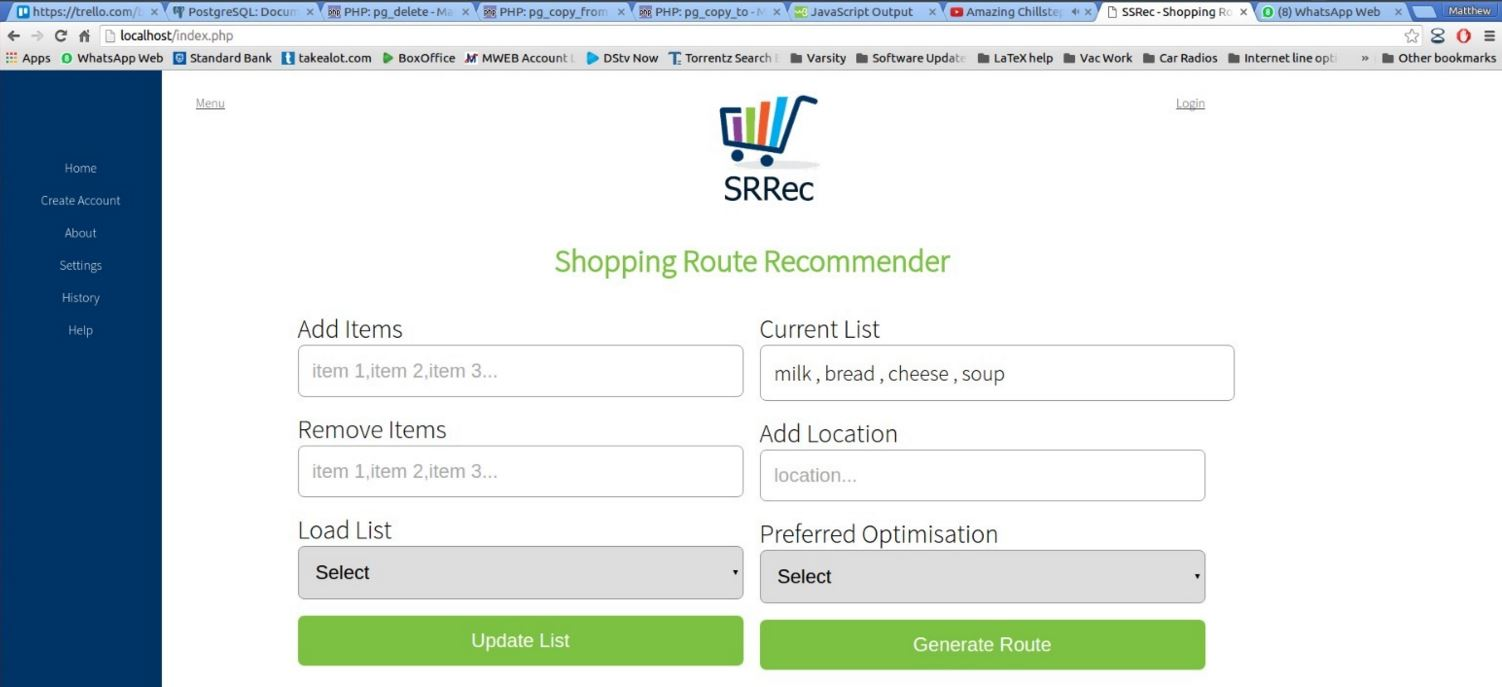
\includegraphics[scale = 0.4]{Images/index_and_menu_page.JPG}
						\label{home page}
					\end{figure}
					
					\item Route and Directions page generated after a user has input their shopping list, location and preferred optimisation:
					\begin{figure}[h!]
						\centering
						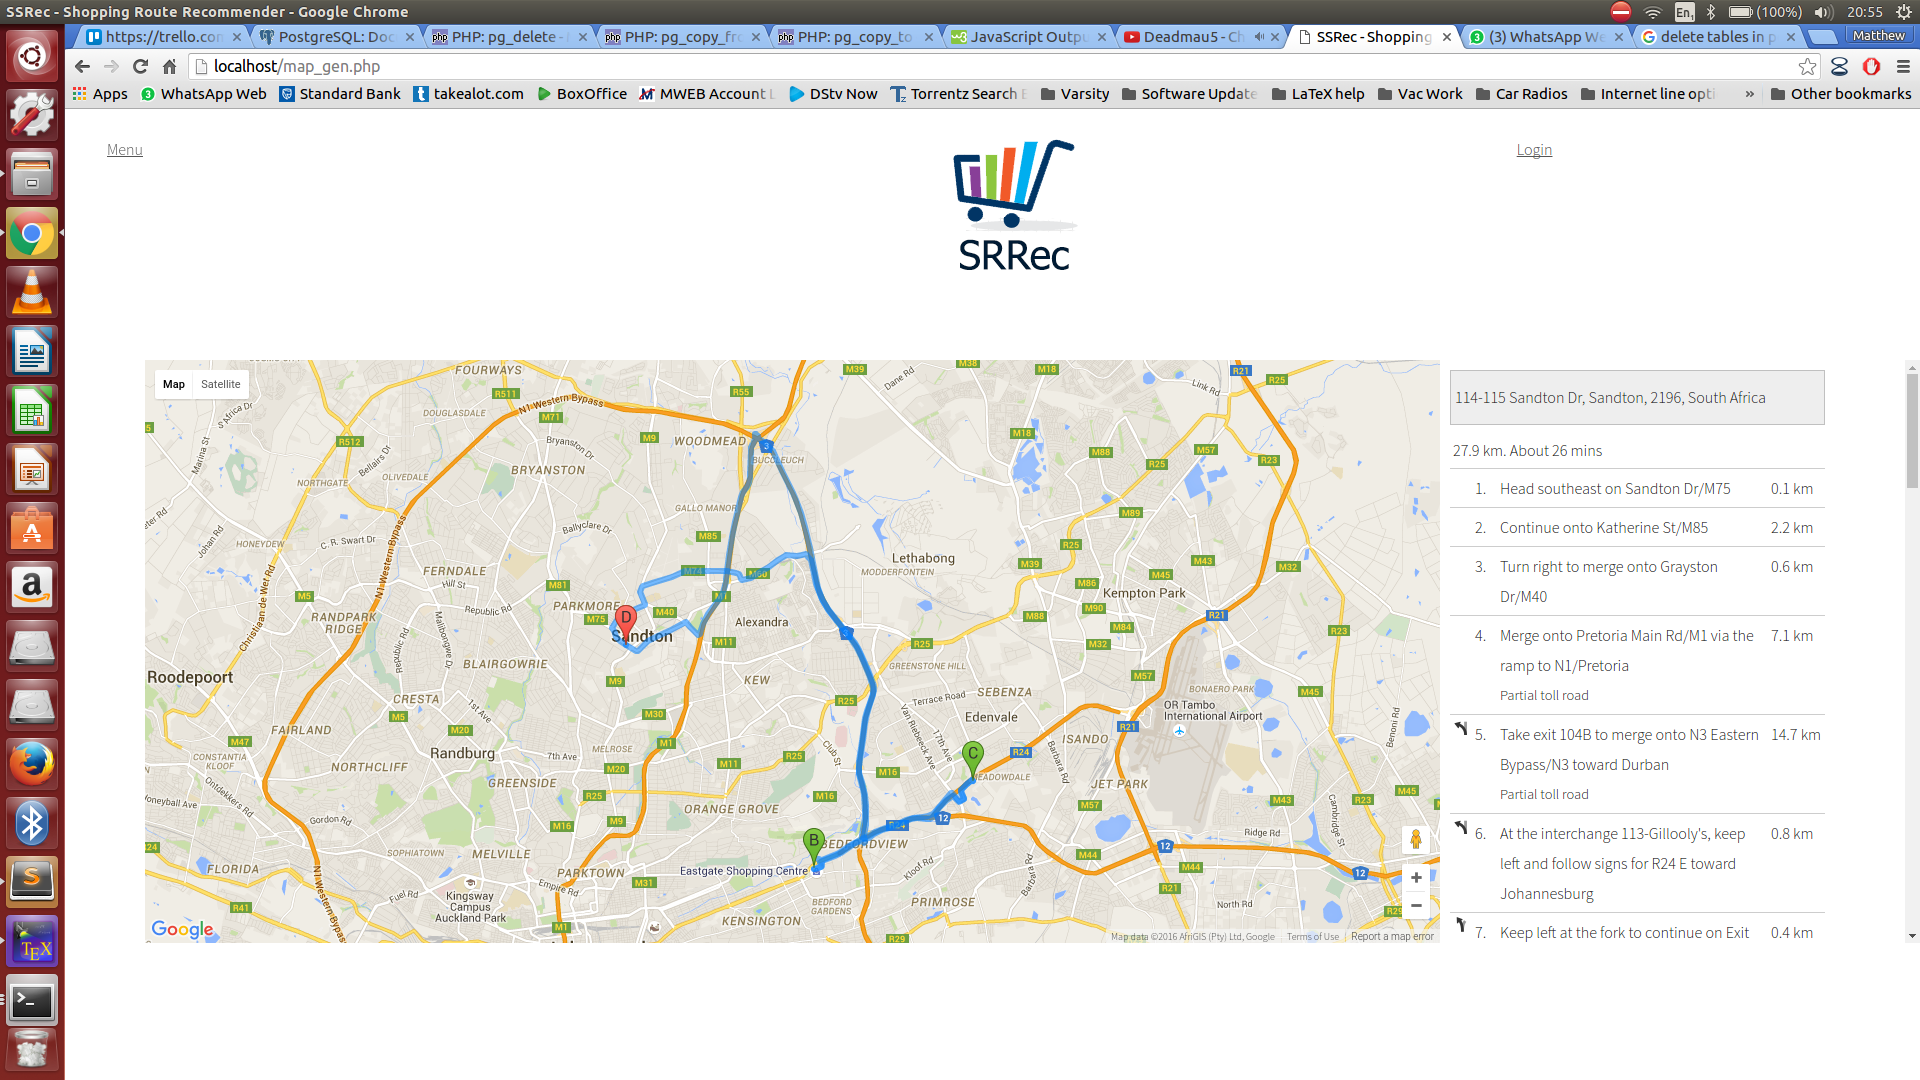
\includegraphics[width =\textwidth]{Images/Map_new.png}
						\label{map page}
					\end{figure}
					
					\newpage
					\item The page where a user can either login or create a new account:
					\begin{figure}[h!]
						\centering
						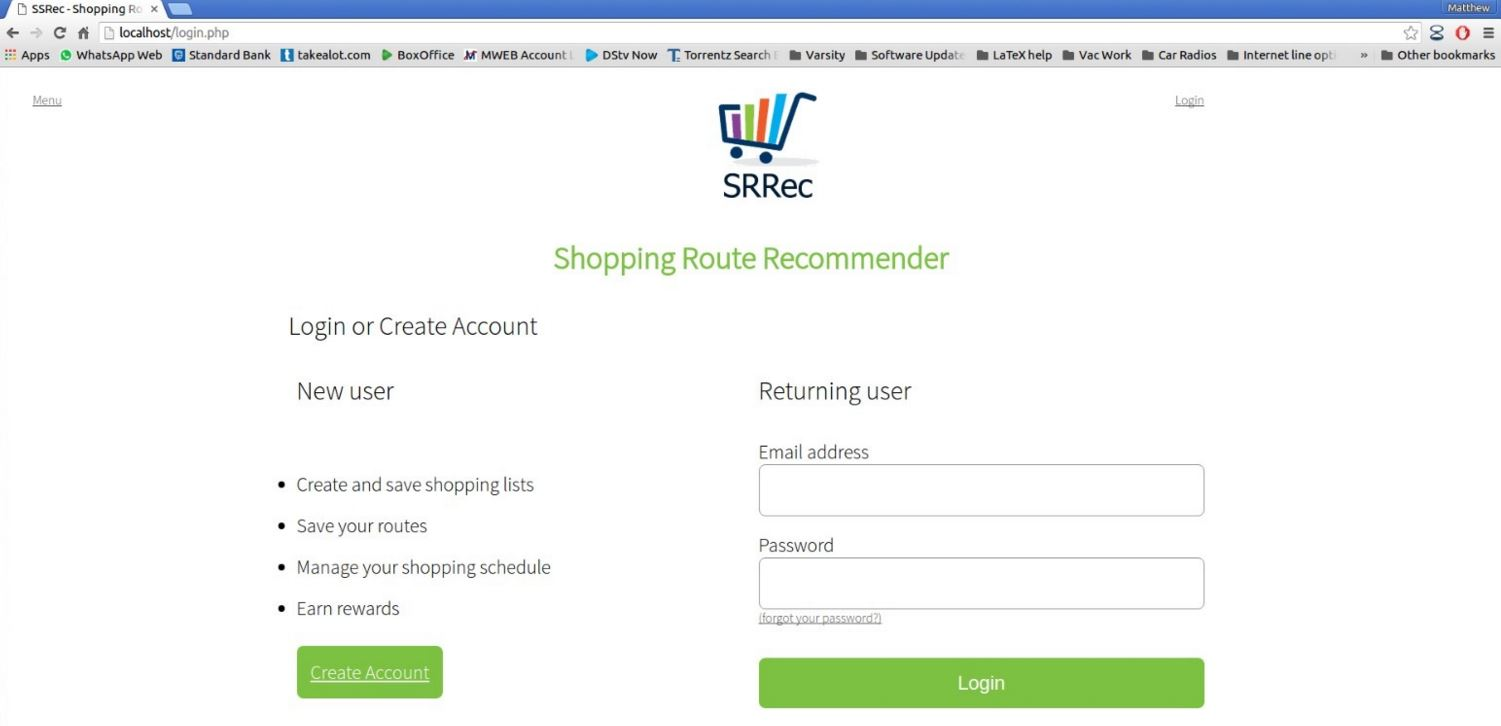
\includegraphics[scale = 0.4]{Images/login_page.JPG}
						\label{login page}
					\end{figure}
					
					
					\item The page where a new user can create an account:
					\begin{figure}[h!]
						\centering
						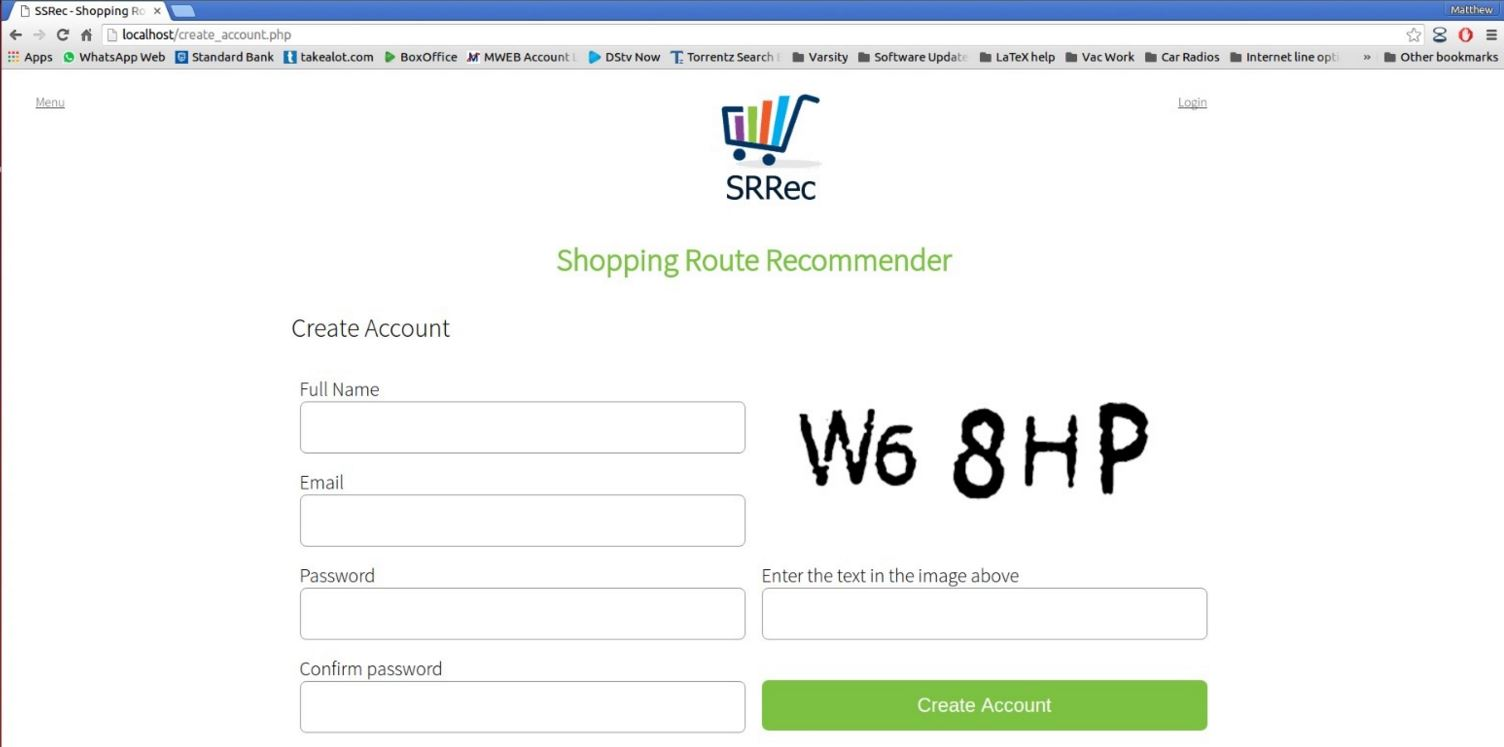
\includegraphics[scale = 0.4]{Images/create_account_page.JPG}
						\label{create account page}
					\end{figure}
													
				\end{itemize}
		
		\subsection{Hardware Interfaces}
		
			The SRRec application does not require nor support any hardware interfaces.
		
		\subsection{Software Interfaces}
		
			SRRec is a web application. Therefore it will be compatible with all operating systems including smartphone and tablet operating systems. It only needs to be compatible on web browsers which support HTML, CSS, JavaScript and PHP. It has been tested on Motzilla, Firefox, Google Chrome, Microsoft Edge and Safari web browsers. \\
			
			Furthermore, the application makes use of the Google Maps API in order to generate and display the map with the optimised shopping route. 
		
		\subsection{Communications Interfaces}
		
			Since SRRec is a web application, network communications are necessary. It runs off a cloud hosted server such that it is readily available with an internet connection so as to communicate with both the user and the Google Maps API. Another communication interface is through the users GPS (if available), which the application uses to locate the nearest shops.
	
	\section{Other Non-functional Requirements}
	
		\subsection{Performance Requirements}
		
			The SRRec is dependent on retrieving only relevant information from multiple large databases. This is to be done in an optimised fashion in order to allow fast data retrieval without unnecessary delays. The application should respond in real-time as the user inputs information.\\
		
			Since the SRRec is a website application, any changes or updates made will be automatically available to the user the next time the website is loaded. Thus SRRec will always be up-to-date.\\
		
			The application should have a maximum range for the shops selected so as not to recommend an infeasible route. It should also be able to still provide a route even if certain items are not available nearby.
		
		\subsection{Safety Requirements}
		
			The application should avoid taking users to the wrong locations, especially if those locations are in dangerous areas. The SRRec should only provide routes along known roads.
		
		\subsection{Security Requirements}
		
			The databases used by SRRec should be protected from random access. User credentials are to be taken in by the application for users to sign into their profiles. Thus there needs to be a secure authentication system. The credentials also need to be safely stored on a secure server to protect them.
		
		\subsection{Software Quality Attributes}
			
			This application incorporates the use of user credentials to allow users to store and access their lists on a 	server without losing their list or having to keep the website active. The application has a simplistic graphical interface that is easy-to-use. The website is easily interpreted and a new user should be able to use the website without requiring any sort of tutorial or explanations.
		
%		\subsection{Other Requirements}
%		
%			\textbf{NOT APPLICABLE TO US YET}
		
	%----------------------------------------------------------------------------------------
	%	REFERENCES
	%----------------------------------------------------------------------------------------
	
	
	
\end{document}